\newpage\pagestyle{main}

\chapter{Gestione della Conoscenza e Memoria a Grafo}\label{chap:second}

\inlineminitoc

% ─────────────────────────────────────────────────────────────────────────────
\section{Limiti dei database vettoriali vs. database a grafo}

La maggior parte dei sistemi di Retrieval-Augmented Generation (RAG) \cite{rag_original} attualmente in uso si basano su database vettoriali per memorizzare e recuperare i documenti indicizzati. Questi database sono progettati per eseguire ricerche di similarità su rappresentazioni vettoriali ad alta dimensionalità, e sono estremamente efficienti nel recuperare frammenti di testo che sono semanticamente vicini alla query dell'utente. Tuttavia, questa efficienza viene ottenuta a costo di una perdita significativa di struttura e contesto.

In un contesto dove la natura dei dati è strutturata e gerarchica, la frammentazione dei dati in chunk indipendenti, porta inevitabilmente alla perdita di coerenza e alla difficoltà di ricostruire il contesto originale. Lo scopo di questo lavoro è proprio quello di risolvere questa limitazione fondamentale, integrando un database a grafo che non solo memorizza i documenti indicizzati, ma anche le relazioni strutturali tra di essi, permettendo così di preservare e sfruttare il contesto in modo molto più efficace durante il processo di recupero delle informazioni.

% ─────────────────────────────────────────────────────────────────────────────
\subsection{Frammentazione e perdita di coerenza}

Il limite prinicipale riguarda la perdita di contesto causata dalla frammentazione dei documenti in chunk indipendenti. In un database vettoriale, ogni chunk viene trattato come un'entità isolata, e la ricerca restituisce solo i chunk che presentano la massima similarità con la query. Quindi risulta quasi impossibile recuperare chunk adiacenti che potrebbero essere essenziali per la corretta generazione della risposta.

Una conseguenza pratica di questa frammentazione è che l'LLM potrebbe ricevere solo una porzione del testo che contiene l'informazione chiave, ma senza il contesto necessario per interpretarla correttamente. Ad esempio, un paragrafo che descrive un protocollo di trattamento medico potrebbe essere restituito come risultato della ricerca, ma senza i paragrafi adiacenti che definiscono la condizione clinica o le controindicazioni, l'LLM potrebbe generare una risposta imprecisa o addirittura pericolosa.

Un secondo problema più sottile è legato alla dipendenza semantica tra i chunk. Il sistema potrebbe restituire un chunk che fa uso di termini tecnici o di abbreviazioni che sono definiti solo in un chunk adiacente, e senza quel chunk l'LLM potrebbe non essere in grado di comprendere il significato del testo restituito. In questo senso, la frammentazione non solo riduce la quantità di informazione disponibile, ma anche la qualità dell'informazione stessa, poiché il contesto è spesso essenziale per interpretare correttamente i dati.

% ─────────────────────────────────────────────────────────────────────────────
\subsection{Relazioni Esplicite vs. Implicite}

In un database vettoriale, le relazioni tra i chunk di testo sono solo implicitamente codificate nella vicinanza dei loro embedding. Non esiste una rappresentazione esplicita delle relazioni strutturali o semantiche tra i diversi pezzi di informazione, e il sistema deve affidarsi alla similarità dei vettori per inferire queste relazioni. Questo approccio è intrinsecamente approssimativo e può portare a risultati incoerenti, soprattutto quando la query dell'utente è formulata in modo da richiedere una comprensione più profonda del contesto o delle relazioni tra i concetti.

In un database a grafo, invece, le relazioni sono esplicitamente rappresentate come archi tra i nodi. Questo significa che possiamo definire relazioni specifiche che codificano in modo deterministico le connessioni tra i diversi elementi della Knowledge Base. Questa rappresentazione esplicita consente al sistema di navigare lungo queste relazioni in modo preciso e predicibile, superando la pura approssimazione statistica degli embedding e permettendo di recuperare informazioni correlate in modo più efficace.

\begin{figure}[H]
    \centering
    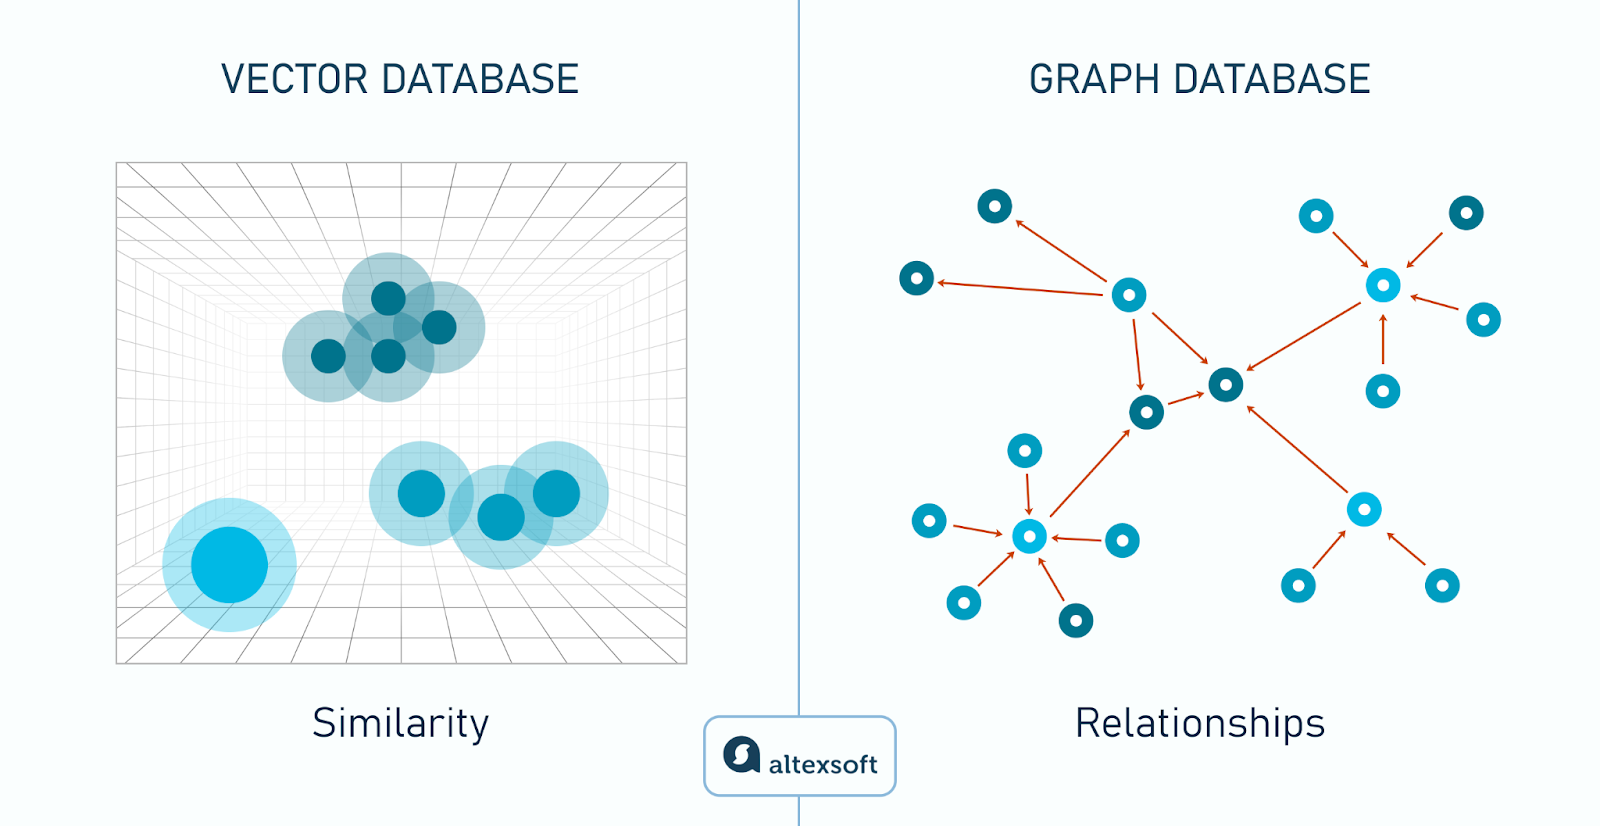
\includegraphics[width=1\textwidth]{_figures/vector_vs_graph_structure.png}
    \caption{Differenza tra memorizzazione lineare e strutturata. Fonte: \url{https://www.altexsoft.com/blog/vector-database/}}
    \label{fig:structure_comp}
\end{figure}

% ─────────────────────────────────────────────────────────────────────────────
\section{Modellazione del Grafo della Conoscenza}

Per questo progetto, è stata utilizzata una struttra dei dati che ha permesso di rappresentare in modo efficace sia il testo dei documenti indicizzati sia le relazioni tra di essi. Il documento non è rappresentato come una stringa piatta, ma come un'entità strutturata con una gerarchia interna precisa. Per ogni documento sono presenti anche molteplici rappresentazioni della stessa informazione, le queli vengono utilizzate per massimizzare la qualità del recupero.

Lo schema del grafo è stato progettato per essere flessibile e scalabile, in modo da poter essere facilmente esteso in futuro con nuovi tipi di nodi o relazioni se necessario. La struttura attuale è stata definita sulla base delle esigenze specifiche del dominio medico, ma i principi di modellazione adottati sono generali e possono essere applicati a qualsiasi dominio in cui la conservazione del contesto e delle relazioni tra le informazioni sia cruciale.

% ─────────────────────────────────────────────────────────────────────────────
\subsection{Schema dei Nodi e delle Relazioni}

Il modello implementato prevede i seguenti tipi di nodo e di relazione:

\begin{itemize}
    \item \textbf{Nodo \texttt{Document}}: Rappresenta l'origine dell'informazione, ovvero il documento sorgente da cui è stato estratto il contenuto. Memorizza il titolo del documento e funge da radice della gerarchia per tutti i paragrafi che lo compongono.

    \item \textbf{Nodo \texttt{Paragraph}}: È l'unità atomica di informazione nel grafo. Contiene il testo integrale del paragrafo, la sua posizione ordinale all'interno del documento \\ (\texttt{document\_position}) e, una volta sincronizzato nello Shard locale, i metadati di utilizzo \texttt{hit\_count} e \texttt{last\_accessed}. La proprietà \texttt{document\_position} è il parametro chiave per il context windowing.

    \item \textbf{Nodo \texttt{Question}}: Rappresenta una domanda tipo che l'utente potrebbe porre per ottenere l'informazione contenuta nel paragrafo collegato. Queste sono state generate automaticamente durante la fase di indicizzazione tramite una chiamata all'LLM. Aggiungere questi nodi consente di migliorare il recuper dei dati, poiché l'utente tenderà a fare domande che saranno di conseguenza più simili alle domande generate, aumentando la probabilità di ottenere un punteggio di similarità elevato durante la ricerca vettoriale.

    \item \textbf{Nodo \texttt{Statement}}: Rappresenta un'affermazione chiave estratta sinteticamente dal paragrafo, anch'essa generata automaticamente dall'LLM durante l'indicizzazione. Mentre le domande rappresentano interrogativi che possono essere associati al paragrafo, le affermazioni rappresentano sintesi assertive del contenuto, e possono essere utili per recuperare informazioni in modo più efficace nel caso di messaggi dell'utente formulati in modo affermativo.

    \item \textbf{Nodo \texttt{Embedding}}: Rappresenta la vera e propria codifica vettoriale di un paragrafo, di una domanda o di un'affermazione. Questi nodi contengono un array di numeri che rappresenta la loro posizione nello spazio vettoriale. La presenza di questi nodi è fondamentale per la ricerca per similarità.

    \item \textbf{Relazione \texttt{HAS\_PARAGRAPH}}: Collega un nodo \texttt{Document} ai suoi nodi \texttt{Paragraph}, codificando la struttura gerarchica del documento. Questa relazione è fondamentale per il context windowing. Data una lista di paragrafi recuperati, il sistema risale al documento genitore e da lì recupera tutti i paragrafi con posizione compresa nell'intervallo di interesse.

    \item \textbf{Relazione \texttt{HAS\_QUESTION}}: Collega un nodo\texttt{Paragraph} alle sue domande associate, permettendo al sistema di navigare bidirezionalmente tra un paragrafo e le interrogazioni che rappresentano il suo contenuto.

    \item \textbf{Relazione \texttt{HAS\_STATEMENT}}: Collega un nodo \texttt{Paragraph} alle sue affermazioni chiave, con lo stesso scopo di \texttt{HAS\_QUESTION} ma per le rappresentazioni di tipo assertivo.

    \item \textbf{Relazione \texttt{HAS\_EMBEDDING}}: Collega un nodo testuale (\texttt{Paragraph}, \texttt{Question} o \texttt{Statement}) al suo embedding vettoriale corrispondente, completando il collegamento tra la rappresentazione simbolica e quella subsimbolica dell'informazione.
\end{itemize}

\begin{figure}[!htbp]
    \centering
    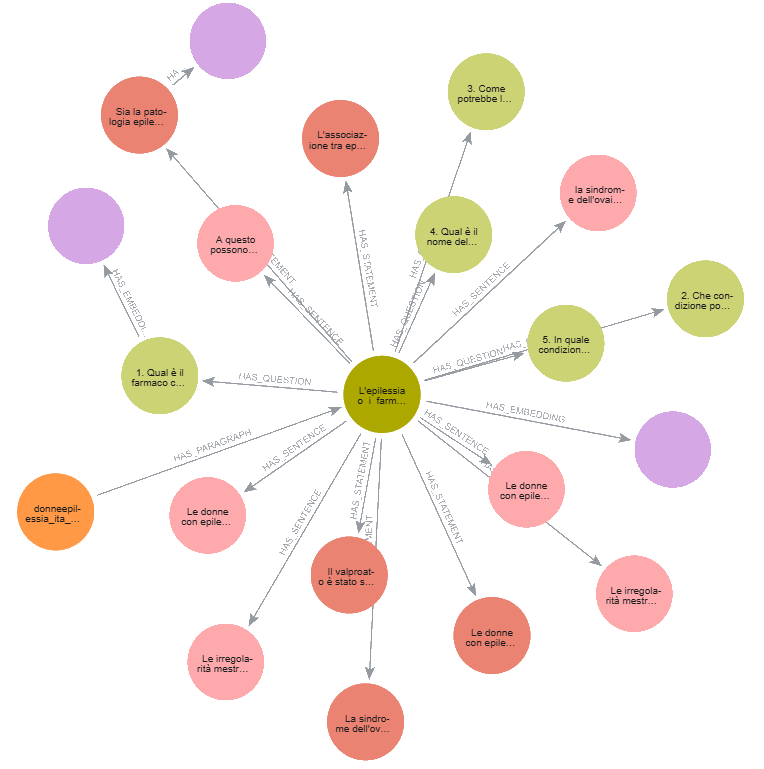
\includegraphics[width=0.95\textwidth]{_figures/graph_metamodel.png}
    \caption{Metamodello del database: nodi \texttt{Document}, \texttt{Paragraph},
        \texttt{Question}, \texttt{Statement} ed \texttt{Embedding} con le rispettive
        relazioni. Il grafo raffigurato è estratto da una porzione della Knowledge Base
        medica relativa al tema dell'epilessia, e mostra come un singolo nodo
        \texttt{Paragraph} sia connesso a più domande, affermazioni ed embedding.}
    \label{fig:metamodel}
\end{figure}

\newpage

% ─────────────────────────────────────────────────────────────────────────────
\section{Rappresentazione Vettoriale e Indicizzazione}

Come spiegato nella sezione precedente, ogni nodo testuale del grafo è collegato a un nodo \texttt{Embedding} che contiene la sua rappresentazione vettoriale. Questa rappresentazione è fondamentale per il processo di recupero, poiché consente di eseguire ricerche per similarità tra la query dell'utente e i contenuti della Knowledge Base. La fase di indicizzazione dei documenti prevede quindi non solo l'estrazione del testo e la creazione dei nodi testuali, ma anche la generazione degli embedding corrispondenti tramite un modello di embedding locale.

% ─────────────────────────────────────────────────────────────────────────────
\subsection{Processo di Embedding con Ollama}

Quando l'utente pone una domanda che necessita di documenti per essere risolta, il sistema deve prima trasformare il testo della query nello stesso spazio vettoriale in cui sono stati proiettati i contenuti della Knowledge Base, in modo da poter calcolare la similarità. Il processo viene eseguito in due operazioni principali:

\begin{enumerate}
    \item Il testo della query viene trascritto da Whisper e inviato al modello di embedding \textit{Embedding-Gemma} \cite{embedding_gemma_2025} in esecuzione locale tramite l'ecosistema \textbf{Ollama} \cite{ollama}. Il modello genera il vettore corrispondente in tempo reale, senza che la query lasci l'infrastruttura locale.

    \item Il vettore della query viene inviato a Neo4j, che esegue una ricerca sul Vector Index configurato sugli embedding della Knowledge Base. Il risultato è una lista ordinata di nodi \texttt{Embedding} con il relativo punteggio di similarità coseno, da cui il sistema risale ai nodi testuali tramite la relazione dedicata.

\end{enumerate}

È importante sottolineare che sia la generazione degli embedding presenti nella Knowledge Base sia la generazione dell'embedding della query avvengono utilizzando lo stesso modello, questo per garantire la massima coerenza nello spazio vettoriale e quindi la massima efficacia nella ricerca per similarità. L'utilizzo di un modello di embedding locale, inoltre, consente di mantenere il controllo completo sui dati e di evitare problemi di latenza o di privacy associati all'invio di query a servizi esterni.

% ─────────────────────────────────────────────────────────────────────────────
\subsection{Vector Index e Similarity Search}

All'interno di Neo4j è stato configurato un \textbf{Vector Index} \cite{neo4j_vector_search} che utilizza l'algoritmo di \textbf{similarità del coseno}. La similarità del coseno misura il coseno dell'angolo tra due vettori nello spazio ad alta dimensionalità, risultando indipendente dalla loro norma e quindi particolarmente adatta a confrontare rappresentazioni testuali, dove la direzione del vettore codifica il significato semantico. Il calcolo della similarità del coseno è espresso dalla seguente formula:

\begin{equation}
    \cos(\theta) = \frac{\mathbf{A} \cdot \mathbf{B}}{\|\mathbf{A}\| \|\mathbf{B}\|}
    \label{eq:cosine}
\end{equation}

dove $\mathbf{A}$ è il vettore del messaggio utilizzato nella query e $\mathbf{B}$ è il vettore del testo ricercato nel database. Un valore di $\cos(\theta)$ pari a 1 indica vettori identici (massima similarità), mentre un valore pari a 0 indica vettori ortogonali (nessuna similarità semantica).

Il sistema esegue una ricerca ordinata per similarità, restituendo i nodi \texttt{Embedding} con i punteggi più alti. Tuttavia, non tutti i risultati vengono considerati validi per la fase di recupero. Viene applicata una soglia di confidenza (80\%) che filtra i risultati in base al loro punteggio di similarità. Questo viene fatto per garantire che solo i risultati più pertinenti vengano utilizzati per la generazione della risposta, evitando che l'LLM si basi su contesti debolmente correlati alla domanda dell'utente, che potrebbero portare a risposte imprecise o fuorvianti. La scelta di questa soglia è stata determinata empiricamente durante la fase di sviluppo, bilanciando la necessità di recuperare informazioni rilevanti con il rischio di includere dati non pertinenti.

% ─────────────────────────────────────────────────────────────────────────────
\section{Strategie di Recupero e Navigazione del Contesto}
\label{sec:context_windowing}

Una volta indivituato il paragrafo ancora tramite la ricerca vettoriale, il sistema non si limita a restituire solo quel singolo paragrafo all'LLM, ma implementa una strategia di \textbf{context windowing dinamico} che consente di recuperare automaticamente i paragrafi adiacenti, creando così un contesto più ampio e coerente per la generazione della risposta.

% ─────────────────────────────────────────────────────────────────────────────
\subsection{Context Windowing Dinamico}

Invece di restituire solo il paragrafo ancora, il sistema risale al nodo \texttt{Document} genitore e recupera tutti i paragrafi con posizione compresa nell'intervallo di $\pm 2$ posizioni rispetto al paragrafo ancora. In questo modo viene creata una finestra di contesto che include fino a cinque paragrafi consecutivi. Questo non solo aumenta l'accuratezza della risposta fornendo più contesto, ma nella formula dello shard utilizzato come cache, consente di predirre domande future che potrebbero essere correlate a quei paragrafi adiacenti, aumentando così la probabilità di cache hit nelle query successive.

La finestra di $\pm 2$ posizioni è stata scelta come compromesso tra la necessità di fornire un contesto sufficiente e il rischio di includere informazioni troppo distanti che potrebbero non essere rilevanti per la domanda dell'utente. Questa strategia consente di mantenere un equilibrio tra la coerenza del contesto e la pertinenza delle informazioni fornite all'LLM, migliorando significativamente la qualità delle risposte generate, ed evitando di incrementare inutilmente la dimensione dello shard locale.

\begin{figure}[H]
    \centering
    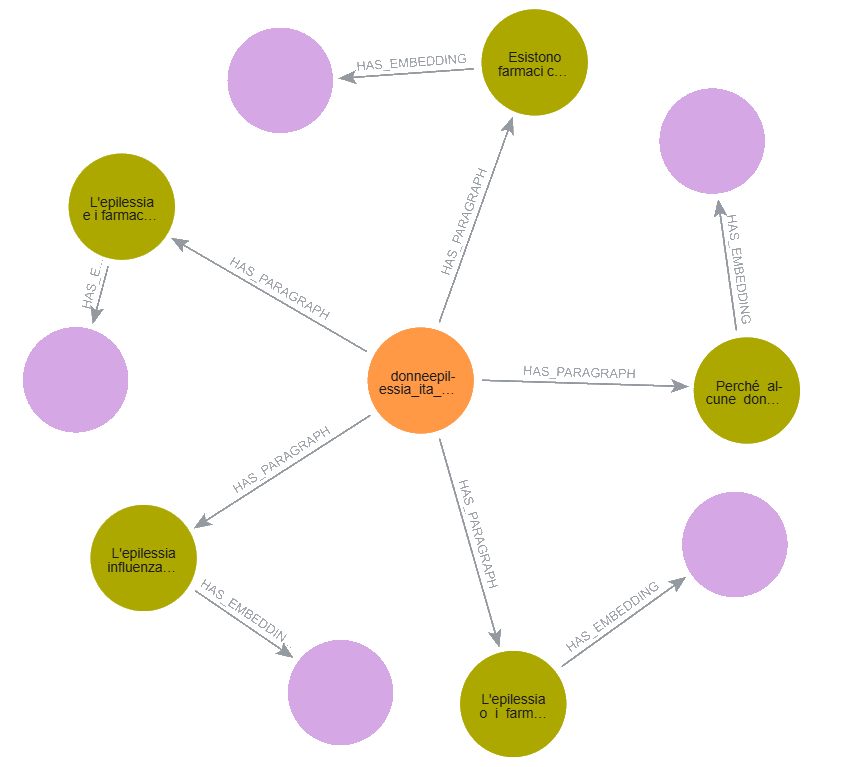
\includegraphics[width=1\textwidth]{_figures/context_expansion_logic.png}
    \caption{Visualizzazione del documento con la finestra di contesto.}
    \label{fig:context_expansion}
\end{figure}

% ─────────────────────────────────────────────────────────────────────────────
\subsection{Vantaggi della navigazione sequenziale}

Questa strategia offre numerosi vantaggi rispetto a un approccio che restituisce solo il paragrafo ancora. Innanzitutto, consente di preservare la coerenza del testo, poiché i paragrafi adiacenti spesso contengono informazioni che si riferiscono direttamente al paragrafo ancora, e che sono essenziali per una corretta interpretazione del contenuto. In secondo luogo, migliora la capacità dell'LLM di generare risposte più accurate e complete, poiché ha accesso ad un contesto più ricco e dettagliato.

I benefici di questo approccio sono particolarmente evidenti in documenti tecnici o medici, dove la comprensione di un concetto dipende strettamente dalle definizioni fornite nelle righe precedenti. Un paragrafo che descrive il protocollo di somministrazione di un farmaco antiepilettco, per esempio, acquisisce significato completo solo se l'LLM ha accesso anche al paragrafo precedente che definisce la condizione clinica per cui quel farmaco è indicato. Con il context windowing, questa informazione è sempre disponibile, indipendentemente da quale paragrafo sia stato il migliore risultato della ricerca vettoriale.

Un ulteriore vantaggio riguarda la robustezza rispetto a domande formulate in modo parziale o indiretto. Anche se il paragrafo ancora non contiene tutte le informazioni necessarie per rispondere, i paragrafi adiacenti spesso le completano, riducendo la probabilità che l'LLM si trovi costretto a dedurre informazioni non presenti nel contesto.

% ─────────────────────────────────────────────────────────────────────────────
\section{Implementazione dello Sharding e Sincronizzazione}

Un aspetto cruciale di questa tesi è il passaggio dei dati dal database remoto allo Shard locale. Questo processo non è una semplice copia dei dati: è una strategia dinamica che tiene traccia dell'utilizzo di ogni nodo nel tempo, e che usa queste informazioni sia per decidere quali dati mantenere in cache sia per garantire che le interrogazioni successive possano essere soddisfatte localmente il più spesso possibile.

% ─────────────────────────────────────────────────────────────────────────────
\subsection{Logica di Hit-Rate}

Ogni volta che un nodo viene recuperato dal database remoto, il sistema non si limita a restituirlo all'LLM come risultato della ricerca, ma lo proietta anche nello Shard locale tramite un'operazione di upsert. Il termine upsert indica una scrittura condizionale. Se il nodo non è ancora presente nello Shard, viene creato con \texttt{hit\_count = 1}, se invece è già presente, vengono aggiornati solo i suoi metadati di utilizzo.

Nello specifico, il sistema incrementa la proprietà \texttt{hit\_count} di una unità e aggiorna la proprietà \texttt{last\_accessed} con il timestamp corrente. Questa proprietà, in combinazione con il timestamp, è fondamentale per la politica di gestione della memoria. I nodi con un alto \texttt{hit\_count} e un timestamp recente sono considerati \textbf{``conoscenza calda''}, ovvero informazioni che l'utente ha consultato frequentemente di recente e che ha quindi alta probabilità di consultare nuovamente nel corso della stessa sessione. Questi nodi hanno la massima priorità di permanenza nello Shard e saranno gli ultimi ad essere rimossi quando si attiva la politica di eviction.

Questa logica di tracciamento dell'utilizzo consente al sistema di adattarsi dinamicamente alle esigenze dell'utente, mantenendo nello shard le informazioni più rilevanti e frequenti, e rimuovendo quelle che sono state consultate meno spesso o che non sono state consultate da molto tempo. In questo modo, lo Shard locale diventa una rappresentazione dinamica e adattiva della conoscenza più pertinente per l'utente, migliorando significativamente la latenza delle risposte e l'efficacia del recupero delle informazioni durante la sessione conversazionale.

\newpage

% ─────────────────────────────────────────────────────────────────────────────
\subsection{Algoritmo di Eviction LFU (Least Frequently Used)}

Per garantire che lo Shard locale non cresca indefinitamente e non saturi la memoria del dispositivo su cui è in esecuzione l'agente, è stata implementata una soglia massima di 30 nodi \texttt{PARAGRAPH}. Questa soglia rappresenta il limite superiore della dimensione della cache locale, e viene monitorata costantemente durante l'esecuzione dell'agente.

Quando il numero di nodi \texttt{PARAGRAPH} nello Shard supera la soglia di 30, viene attivata automaticamente una procedura di pulizia che ha lo scopo di riportare il numero di nodi alla soglia, rimuovendo il numero minimo di nodi necessario. La procedura di pulizia si basa su un algoritmo di eviction denominato \textbf{Least Frequently Used (LFU)}, che privilegia la rimozione dei nodi acceduti con minore frequenza.

Questa politica è stata scelta perché si adatta meglio alla natura delle sessioni conversazionali mediche, dove un paziente che chiede più volte informazioni sullo stesso argomento indica un interesse consolidato per quel topic, e i dati correlati devono rimanere in cache anche se non sono stati acceduti nell'ultima query. Al contrario, nodi che sono stati consultati solo una volta o che non sono stati consultati da molto tempo hanno una probabilità molto più bassa di essere rilevanti per le domande future, e quindi vengono rimossi per fare spazio a nuove informazioni più pertinenti.